\documentclass[a4paper,12pt]{report}
\usepackage[utf8]{inputenc} % Kodierung
\usepackage[ngerman]{babel} % Sprache
\usepackage{geometry} % to change the page dimensions
\geometry{left=2.5cm, right=2cm, top=3cm, bottom=3cm} % or letterpaper (US) or a5paper or....
% \geometry{margin=2in} % for example, change the margins to 2 inches all round
% \geometry{landscape} % set up the page for landscape
%   read geometry.pdf for detailed page layout information
\usepackage{graphicx}
\usepackage{float}
\usepackage{fancyhdr}
\usepackage[bottom,hang]{footmisc}
\usepackage{tabularx}
\usepackage{setspace} % Paket für Zeilenabstand
\usepackage{acronym} % Paket für Abkürzungsverzeichnis
\usepackage[numbers,square]{natbib} % numbers ist notwendig für alphadin, squar sorgt für eckige Klammern
\usepackage{url}

%\setlength{\textwidth}{14cm}
%\setlength{\textheight}{25.5cm}
%\setlength{\topmargin}{-2.0cm}
%\setlength{\oddsidemargin}{0cm}
%\setlength{\evensidemargin}{0cm}

\fancypagestyle{plain}{
\fancyhead{}
\renewcommand{\headrulewidth}{0.0pt}}

\pagestyle{fancy}
\renewcommand{\chaptermark}[1]{\markboth{#1}{}}
\fancyhf{}
\fancyhead[R]{}
\fancyhead[L]{\textbf{\nouppercase\leftmark}}
\fancyfoot[R]{\thepage}
\fancyfoot[L]{}
\renewcommand{\headrulewidth}{0.5pt}

% 1.5 facher Zeilenabstand
\onehalfspacing
% weniger Silbentrennung aber dafür mehr Wortzwischenräume
\sloppy

\begin{document}

%===================================================================== Titlepage
\begin{titlepage}
\centering
\vfill
{\bfseries\Huge Masterarbeit}\\[2cm]
{\bfseries\Large Modellierung der Qualitätsmanagementprozesse}\\[0.2cm]
{\bfseries\Large für die Marktüberwachung und Vigilanz in der}\\[0.2cm]
{\bfseries\Large Entwicklung von Medizinprodukten unter}\\[0.2cm]
{\bfseries\Large Berücksichtigung der MDR EU 2017/745}\\
\vfill
vorgelegt von
\vfill
{\large Jens Noack}\\
\vfill
in Kooperation mit der\\[1cm]
{\large W.O.M. WORLD OF MEDICINE GmbH}\\[1cm]
\begin{center}
\begin{minipage}[c]{0.3\textwidth}
   
\includegraphics[width  = 3cm]{Images/wom_logo}
  \end{minipage}
\begin{minipage}[c]{0.2\textwidth}
   
\includegraphics[width  = 3cm]{Images/akad_logo}
  \end{minipage}
\end{center}
\vfill
\begin{center}\parbox{0cm}{\begin{tabbing}
xxxxxxxxxx \= xxxxxxxx \kill
Hochschule:\quad\quad\quad\quad\quad\quad\quad\quad\quad \= AKAD Bildungsgesellschaft \\
Studiengang: \> Wirtschaftsingenieurwesen \\
\> Master of Engineering \\
Matrikelnummer: \> 2929271 \\
Erstgutachter: \> Dr. Andrea Herrmann\\
Betreuer Firma: \> Dr. Jan Bischof
\end{tabbing}}
\end{center}
\end{titlepage}

%===================================================================== Kurzfassung
\addcontentsline{toc}{chapter}{Kurzfassung} %sorgt für Eintrag ins Inhaltsverzeichnis
\chapter*{Kurzfassung} %  *-> erstellt unnummeriertes chapter

Kurzfassung

%===================================================================== Verzeichnisse
\tableofcontents %Inhaltsverzeichnis
\listoffigures %Abbildungsverzeichnis
\listoftables %Tabellenverzeichnis
\chapter*{Abkürzungsverzeichnis} %  *-> erstellt unnummeriertes chapter
\begin{acronym}[XXXXX] %Option in eckigen Klammern ist längste Abkürzung
 \acro{BPM}{Business Process Management}
 \acro{BPMN}{Business Process Model and Notation}
 \acro{EPK}{Ereignisgesteuerte Prozesskette}
 \acro{PMS}{Post Market Surveillance}
 \acro{UML}{Unified Modeling Language}
\end{acronym}

%===================================================================== Einleitung
\chapter{Einleitung}\label{chap:Einleitung}

%===================================================================== Cahpter 2
\chapter{Grundlagen}\label{chap:Grundlagen}
In diesem Kapitel werden wichtige Grundlagen für das Verständnis der Zusammenhänge und die Einordnung der Bedeutung der folgenden Kapitel vermittelt. Dazu wird zunächst das Themenfeld der Geschäftsprozessmodellierung grob beleuchtet, wobei mit BPMN 2.0 eine Modellierungssprache vorgestellt wird, die für die Visualisierung und Modellierung von Geschäftsprozessen im Rahmen dieser Arbeit verwendet wird. Anschließend wird der regulatorische Rahmen auf dem Medizinproduktemarkt sowie die dort vorherrschenden Anforderungen an die Qualitätsprozesse nach der Markteinführung vorgestellt.

\section{Analyse, Visualisierung und Modellierung von Geschäftsprozessen}\label{sec:BPM}
Dieses Kapitel beinhaltet einen groben Überblick über die Grundlagen für das Management von Geschäftsprozessen. Es stellt somit in gewisser Weise das "`Handwerkszeug"' für die gestellte Aufgabe dar, da die Analyse und Anpassung von Geschäftsprozessen einen essentiellen Anteil am Hauptziel dieser Arbeit einnimmt.
\subsection{Business Process Management}\label{subsec:BPManagement}
Zur Beschreibung von Business Process Management kursieren Definitionen von zahlreichen Autoren \citep[vgl.][S. 1]{Freund2014}. An dieser Stelle wird die sehr passende Definition der European Association of BPM (EABPM) vorgestellt, die in der deutschen Übersetzung des Standardwerkes "`BPM Common Body of Knowledge"' \cite[S. 38ff.]{Eabpm2009} folgendermaßen lautet:

\begin{quote}
Die englische Bezeichnung "`Business Process Management"' oder BPM wird synonym verwendet für Geschäftsprozessmanagement oder auch einfach Prozessmanagement. Als Prozess wird eine Reihe von festgelegten Tätigkeiten (Aktivitäten, Aufgaben) definiert, die von Menschen oder Maschinen ausgeführt werden, um ein oder mehrere Ziele zu erreichen. Letztlich geht es darum, einen Kundennutzen zu schaffen und damit auch für das Unternehmen Wert zu generieren.

Business Process Management (BPM) ist ein systematischer Ansatz, um sowohl automatisierte als auch nicht-automatisierte Prozesse zu erfassen, zu gestalten, auszuführen, zu dokumentieren, zu messen, zu überwachen und zu steuern und damit nachhaltig die mit der Unternehmensstrategie abgestimmten Ziele zu erreichen. BPM umfasst die bewusste und zunehmend IT-unterstützte Bestimmung, Verbesserung, Innovation und Erhaltung von End-to-end-Prozessen.
\end{quote}

Im rein betriebswirtschaftlichen Sinne bezeichnet \ac{BPM} somit die Implementierung einer Managementphilosophie, die Unternehmensprozesse als zentralen Erfolgsfaktor eines Unternehmens betrachtet. In Zeiten von Globalisierung, Digitalisierung und dem damit verbundenen permanent ansteigenden Konkurrenzdruck konzentrieren sich Firmen immer mehr auf ihre eigenen Stärken und nutzen das Geschäftsprozessmanagement zur prozessorientierten Gestaltung der Unternehmensstrukturen. Zu den Hauptaufgaben des \ac{BPM} gehören neben dem Dokumentieren auch das Gestalten und Verbessern von Geschäftsprozessen. Dabei wird im Allgemeinen auf standardisierte Modellierungssprachen zurückgegriffen (z.B. UML, EPK oder BPMN), weswegen die IT-Unterstützung für \ac{BPM} eine große Rolle spielt \citep[vgl.][S. 1ff.]{Becker2009}. 

Mit Hilfe von \ac{BPM} ist es Unternehmen möglich ihre Prozesse zu optimieren, so dass diese weniger kosten und schneller werden, wobei trotzdem die Genauigkeit gesteigert wird. Gut angepasste und "`schlanke"' Prozesse sind zudem flexibler und erlauben schneller auf den Markt zu reagieren. Das Ergebnis sind geringere Kosten und eine höhere Kundenzufriedenheit und somit eine bessere allgemeine Performance des Unternehmens. Der Erfolg und die Nachhaltigkeit dieses Konzeptes wird durch die konsequente Einführung von Metriken zur Bestimmung der Leistungsfähigkeit der Prozesse untermauert. Dies ermöglicht schnelle Anpassungen auf neue Situationen, was bei der heutigen Marktdynamik nahezu überlebenswichtig ist \citep[vgl.][S. 7]{Brocke2014}.

Eines der wichtigsten Grundprinzipien von \ac{BPM} ist die permanente Überwachung und Anpassung der Prozesse \citep[S. 11f.]{Brocke2014}. Wie in Abbildung \ref{process_management_cycle} ersichtlich ist, kann das Standardvorgehen bei \ac{BPM} durch einen geschlossenen Zyklus dargestellt werden, in dessen Verlauf ein Prozess ständig analysiert und auf Abweichungen von den Zielen überprüft wird, um entsprechende Änderungen einzuleiten.
\begin{figure}[ht]
\centering
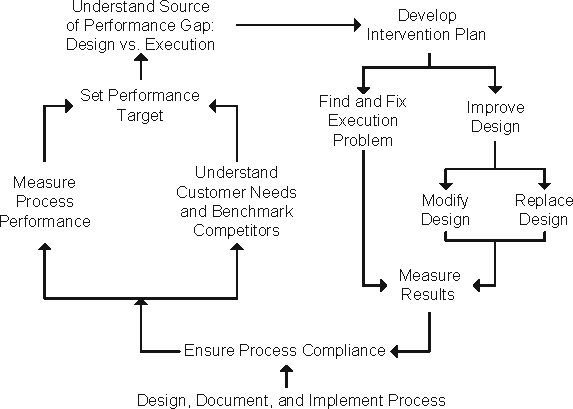
\includegraphics[width=0.8\textwidth]{Images/process_management_cycle}
\caption[Essentieller Zyklus der Geschäftsprozessmodellierung]{Essentieller Zyklus der Geschäftsprozessmodellierung \citep[S. 5]{Brocke2014}}
\label{process_management_cycle}
\end{figure}
\subsection{Business Process Mapping und Business Process Modeling}\label{subsec:BPMappingModeling}
Die Ermittlung und Visualisierung von Geschäftsprozessen stellt eine Teildisziplin im Management von Geschäftsprozessen dar. Gleichzeitig ist sie der Schlüssel zur Anpassung der Geschäftsprozesse, da ein genaues Verständnis der Abläufe für die Anpassung und Verbesserung unerlässlich sind \cite[vgl.][S. 6]{Jacka2009}. Mit dieser Problemstellung befassen sich sowohl Business Process Mapping als auch Business Process Modeling. Der Unterschied zwischen beiden besteht im wesentlichen in der Zielstellung und der damit verbundenen Abstraktionsebene \cite[vgl.][]{Smartdraw}. Process Mapping zielt im Kern auf die Dokumentation eines bestehenden Prozesses ab, weswegen das Unternehmen auf makroskopischer Sicht analysiert wird. Dabei werden die wesentlichen Funktionen und Rollen bei der Transformation des Inputs zum Output betrachtet. Process Modeling hingegen versucht bestehende Prozesse im Detail zu analysieren, um Engpässe aufzudecken und die Effizienz durch Anpassungen zu steigern \cite[vgl.][]{Appian}. Aus diesem Grund sind die dabei entstehenden Modelle detaillierter. Beide Disziplinen verwenden dabei im Idealfall standardisierte Beschreibungssprachen, wobei sich aus der höheren Detailtiefe beim Process Modeling eine höhere notwendige Komplexität der Beschreibungssprache ergibt. Aufgrund der vielen inhaltlichen und methodischen Überschneidungen der beiden Disziplinen kommt es leider häufig zu Verwechslungen beziehungsweise zur synonymen Verwendung beider Bezeichnungen \cite[vgl.][]{Smartdraw}.

Zu den allgemeinen Vorteilen von Process Mapping zählen die bessere Dokumentation der Prozesse, die Möglichkeit den Prozess grafisch zu visualisieren sowie die komplette Sicht auf die vielen verschiedenen Aspekte eines Prozesses \cite[vgl.][S. 8]{Jacka2009}. Neben diesen offensichtlichen Vorteilen gibt es allerdings noch zahlreiche weitere positive Aspekte, deren Wirkungsweise sich erst auf den zweiten Blick erschließt. Beispielsweise erhöht sich die Transparenz der Unternehmensprozesse, wodurch jeder Prozessteilnehmer seine Rolle im kompletten Kontext besser einschätzen kann. Dadurch wird die Wirkung der eigenen Tätigkeiten wesentlich klarer, was das Stolzgefühl der Mitarbeiter stärkt und so zu einer allgemeinen Steigerung der Mitarbeiterzufriedenheit führt. Zudem kann jeder Teilnehmer wesentlich mehr zur stetigen Verbesserung der Prozesse beitragen, da jedem ein holisitischer Blick auf den Prozess gewährt wird. Ein weiterer positiver Nebeneffekt ist die sich zwangsläufig ergebende Kundenorientierung, da für ein sinnvolles analysieren der Prozesse der Blick auf den für den Kunden generierten Output notwendig ist \cite[vgl.][S. 8-11]{Jacka2009}.

\subsection{BPMN 2.0}\label{subsec:BPMN}

\section{Regulatorische Anforderungen für Medizingeräte}\label{sec:RegRequ}

\subsection{Gründe und Bedeutung der Regulierung für Medizinprodukte}\label{subsec:Gruende}
\subsection{Überblick über die wichtigsten Normen}\label{subsec:UeberblickNormen}
\subsection{Auswirkungen auf die Entwicklung und den Produktlebenszyklus}\label{subsec:AuswirkungenAufEntwicklung}
\subsubsection{Requirements Engineering}
\subsubsection{Product Lifecycle Management}

\section{Qualitätsprozesse nach Markteinführung medizinischer Geräte}\label{sec:PMProzesse}
\subsection{Vigilance System}\label{subsec:Vigilance}
\subsection{Post Market Surveillance}\label{subsec:PMS}
\subsection{Post Market Clinical Follow-Ups}\label{subsec:PMCF}
\subsection{Integration in die Entwicklungsprozesse}\label{subsec:IntegrationInDevProzesse}

%===================================================================== Chapter 3
\chapter{Aufnahme des Status Quo}\label{chap:AufnahmeStatusQuo}

%===================================================================== Cahpter 4
\chapter{Anpassung des Prozesses unter Berücksichtigung der Medizinprodukteverordnung (MDR) EU 2017/745}\label{chap:AnpassungAnMDR}

%===================================================================== Chapter 5
\chapter{Integration und Umsetzung des neu modellierten Prozesses}\label{chap:Integration}

%===================================================================== Zusammenfassung
\chapter{Zusammenfassung}\label{chap:Zusammenfassung}

%===================================================================== Diskussion
\chapter{Diskussion}\label{chap:Diskussion}

%===================================================================== Vorlagen
%\chapter{}\label{chap:}
%\section{}\label{sec:}
%\subsection{}\label{subsec:}
%\subsubsection{Requirements Engineering}  -- besitzt keine Nummerierung und taucht nicht im toc auf
%\cite[S. X]{<reference>}
%\ac{<Abkürzung>}

%===================================================================== Literaturverz.
\bibliography{literatur}
\bibliographystyle{alphadin}
%\bibliographystyle{abbrv}
% Übersicht unter: https://de.wikibooks.org/wiki/LaTeX-W%C3%B6rterbuch:_bibliographystyle

%===================================================================== Anhang
\appendix
\chapter[Anhang]{}
\newpage
\section{Anhang 1}

%===================================================================== Eidessattl. Vers.
\chapter*{Eidesstattliche Versicherung} %  *-> erstellt unnummeriertes chapter
Ich versichere, dass ich vorliegende Arbeit selbstständig verfasst, keine anderen als die angegebenen Quellen und Hilfsmittel benutzt sowie alle wörtlich oder sinngemäß übernommenen Stellen in der Arbeit gekennzeichnet habe.
\\[2cm]
\noindent\rule{0.35\textwidth}{0.3pt}\rule{0.2\textwidth}{0pt}\rule{0.45\textwidth}{0.3pt}
\\Ort, Datum\rule{0.418\textwidth}{0pt}Unterschrift
\end{document}